\documentclass[aspectratio=169]{beamer}
\usepackage[utf8]{inputenc}

\usepackage{listings}

\lstset{
    basicstyle=\linespread{1}\scriptsize\ttfamily, 
    numbers=left,
    stepnumber=1,
    showstringspaces=false,
    columns=fullflexible,
    tabsize=2,
    frame=single,
    breakatwhitespace=true,  
    breaklines=true,
    captionpos=b, 
    numberstyle=\tiny,
}

\usetheme{default}
\usecolortheme{seahorse}
\setbeamertemplate{navigation symbols}{}

\AtBeginSection[]
{
    \begin{frame}
        \frametitle{Table of Contents}
        \tableofcontents[currentsection]
    \end{frame}
}

\setbeamertemplate{section in toc}[sections numbered]
\setbeamertemplate{subsection in toc}[subsections numbered]

\title{Intorduction to Optimization}
\subtitle{Scientific Computing}
\author{Stefan Abi-Karam}
\date{Summer 2023}


\begin{document}

\begin{frame}
    \titlepage
\end{frame}

\begin{frame}{Table of Contents}
    \tableofcontents
\end{frame}

\section{Foundations of Optimization}

\begin{frame}{Big Picture}
    Every optimization at a very general level can be viewed as the following:
    \begin{itemize}
        \item I have a set of inputs I can change: $x$
        \item I have a system I plug these inputs into: $f$
        \item The system has an output: $f(x)$
    \end{itemize}

    \vspace{\baselineskip}

    \begin{center}
        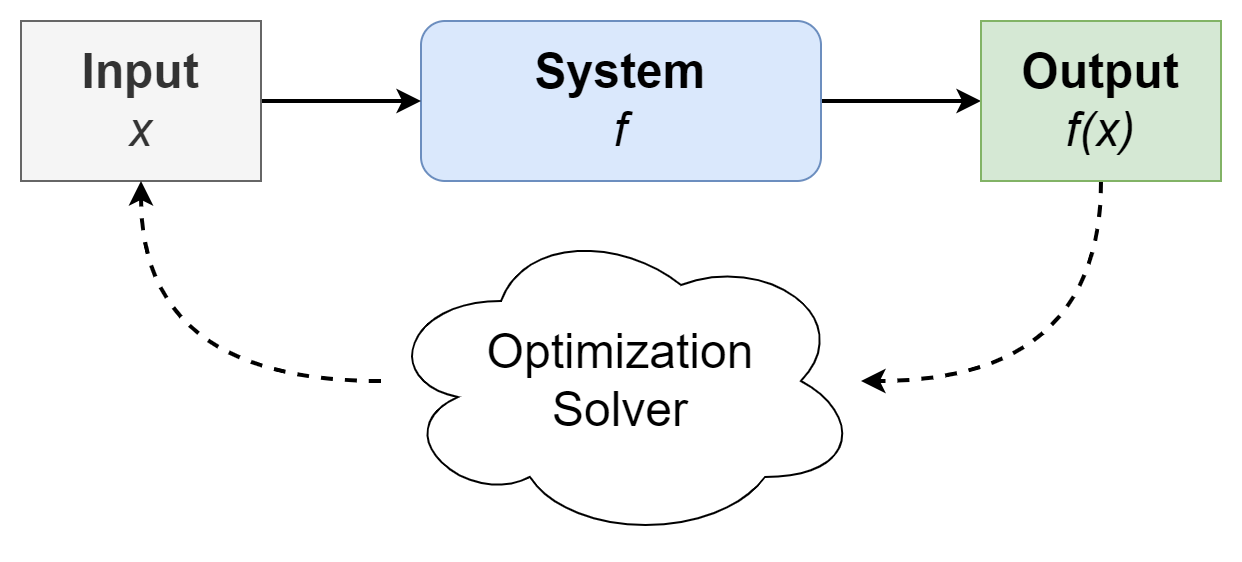
\includegraphics[width=0.5\textwidth]{./imgs/opt_system.png}\\
        \textbf{The goal of evey optimization problem is to find the inputs that give you the "best" output.}
    \end{center}
\end{frame}

\begin{frame}{Big Picture}
    Nost optimization problems are formulated as \textbf{minimization} problems:
    \begin{itemize}
        \item I want to find the inputs that give me the smallest output: $x^* = \arg\min_x f(x)$
    \end{itemize}

    \vspace{\baselineskip}

    Sometimes I want the output to be as big as possible or as close to a target value as possible. We just reformulate these as minimization problems:
    \begin{itemize}
        \item I want to find the inputs that give me the largest output: $x^* = \arg\min_x -f(x)$
        \item I want to find the inputs that give me the output closest to a target value $T$: $x^* = \arg\min_x \mathrm{L}(f(x), T)$, example: $x^* = \arg\min_x |f(x) - T|$
    \end{itemize}
\end{frame}

\begin{frame}{Big Picture}
    We can also include \textbf{constainst} on our input variables that match with real-world descriptions of the problem.
    A problem can have no constraints, one constraint, or multiple constraints of different types.
\end{frame}


\begin{frame}{Big Picture}
    \textbf{Inequality Constraints}: input variables are constaned by $<$, $>$, $\le$, and $\ge$ using inequalities.
    \begin{gather}
        5.99x_1 + 2.99x_2 \ge 10\\
        0 \ge 10 -5.99x_1 - 2.99x_2
    \end{gather}
    Real Example: The minimum order price for ordering parts is $10.00$, I order $x_1$ units of item 1 and $x_2$ units of item 2 is .
    \vspace{\baselineskip}

    \textbf{Equality Constraints}: input variables are constrained by $=$ using equations
    % example: $x_1 + x_2 = 1$
    \begin{gather}
        x_1 x_2 = 70\\
        0 = 70 - x_1 x_2
    \end{gather}
    Real Example: The area of my rectangle that has width $x_1$ and height $x_2$ must be equal to 1.
    \vspace{\baselineskip}
\end{frame}

\begin{frame}{Big Picture}
    \textbf{Numeric Type Constraints}: input variables must be of a certain numeric type
    \begin{gather}
        x_1 \in \{0, 1\}\\
        x_2 \in \mathbb{Z}\text{ (Integers)}\\
        x_3 \in \mathbb{R}\text{ (Real Numbers)}
    \end{gather}
    \vspace{\baselineskip}
\end{frame}

\begin{frame}{Big Picture}
    I may also have multiple outputs that I want to minimize at the same time, known as \textbf{multi-objective optimization}:
    \begin{itemize}
        \item I want to find the inputs that give me the smallest outputs: $x^* = \arg\min_x f_1(x), f_2(x), \dots, f_n(x)$
    \end{itemize}

    \vspace{\baselineskip}

    Multi-objective optimization is a bit more complex since you may have to figure out how to balance which output functions are more important than others. As you change the inputs, one output may improve while another worsens. There are more advanced techniques that solve this issue in different ways.

    \vspace{\baselineskip}

    One simple example is to just minimize the weighted sum of all the outputs where you pick the weights yourself:
    \begin{equation}
        f(x) = w_1 f_1(x) + w_2 f_2(x) + \dots + w_n f_n(x)
    \end{equation}
\end{frame}

\begin{frame}{Big Picture}
    There are many labels you can use to descibe your optimizaton problem:
    \begin{itemize}
        \item Linear / Linear Programming
        \item Non-Linear Optimization
        \item Combinatorial Optimzaiton
        \item Mixed-Integer Optimization
        \item SAT: Boolean Satifiabiley Problem
        \item Multi-Obejecttive Optimization
        \item Balckbox Optimization
        \item Diffeienable Optimzation
    \end{itemize}
\end{frame}

\begin{frame}{Real World Problems}
    To apply optmization to a real-world problem, we must first \textbf{"translate"} the real-world problem to to optmization problem.
    \vspace{\baselineskip}

    All optimzation problems can be described using a common "mathmatical description" we define later.
    \vspace{\baselineskip}

    One weird thing is that there are multiple ways to translate the same problem into different "mathmatical descriptions" that are all valid. However some fomulations of the same problem are easier to solve and analyze than other formulations, even for computer solvers.
\end{frame}

\begin{frame}{Real World Problems}
    % simple linear optimization example

    \textbf{Problem}: I have $x_1$ pounds of flour and $x_2$ pounds of sugar. I want to maximize the profit I make from selling these material. I set the price of flour to $5.99$ per pound and the price of sugar to $2.99$ per pound. The wholesale cost of flour is $2.00$ and the wholesale cost of flour is $1.00$. I have a total of $10.00$ to spend on these items. Assume I can sell all the items I buy.

    \vspace{\baselineskip}

    \textbf{Formulation}:
    \begin{align}
        \max f(x_1, x_2) & = 5.99x_1 + 2.99x_2 - 2x_1 - x_2 \\
                         & \text{subject to}                \\
        0                & \ge 10 -5.99x_1 - 2.99x_2        \\
        0                & \le x_1, x_2
    \end{align}

    \begin{center}
        This is a simple linear optimization problem.
    \end{center}

\end{frame}


\begin{frame}{Real World Problems}
    \textbf{Problem}: You are planning a field trip for your class and need to assign hotel roommates for the trip. You have $n$ students (assume and even number of students) and two studetns will share one room, so you need $n/2$ rooms. Each student has ranked evey other student in order of preference for roomates. As a good enough solution, you need to assign the pairs of people so the final solution is "stable": there are no two people which are not roommates and which both prefer each other to their roommate as opposed to their assigned match.

    \vspace{\baselineskip}

    \textbf{Formulation}: There is more than one way to formulate this problem as an optimization, but this problem actually has a deterministic solution that doesnt need an optimization algorithm to solve. There is also no guarentee that there will always be a "stable" solution.

    \begin{center}
        This is a combinatorial optimization problem.
    \end{center}

\end{frame}

\end{document}